\documentclass[12pt, oneside]{report}   	% use "amsart" instead of "article" for AMSLaTeX format
\usepackage{geometry}                		% See geometry.pdf to learn the layout options. There are lots.
\geometry{a4paper}                   		% ... or a4paper or a5paper or ... 
%\geometry{landscape}                		% Activate for for rotated page geometry
%\usepackage[parfill]{parskip}    		% Activate to begin paragraphs with an empty line rather than an indent
\usepackage{graphicx}				% Use pdf, png, jpg, or eps§ with pdflatex; use eps in DVI mode
\usepackage{float}					% TeX will automatically convert eps --> pdf in pdflatex

\usepackage{amssymb}
\usepackage[utf8]{inputenc}
\usepackage[german]{babel}

%\usepackage{fancyhdr}
%\pagestyle{fancy}

%\fancyhead{}
%\fancyfoot{}

%\interfootnotelinepenalty=10000

\title{Twitter Sentiment Analyse}
\author{Jérémie Blaser, Nicolas Roos\\
	ZHAW (Zürcher Hochschule für Angewandte Wissenschaften),\\
	Zürich,\\
	Switzerland,\\
	\texttt{blaseje1@students.zhaw.ch},
	\texttt{roosnic1@students.zhaw.ch}}
\date{\today}							% Activate to display a given date or no date


%\fancyhead[C] {End-2-End Services/Monitoring}
%\fancyfoot[C] {Seite \thepage}
%\fancyfoot[L] {Nicolas Roos}
%\fancyfoot[R] {\today}


\begin{document}
\maketitle


%\paragraph{Ansprechpartner an der ZHAW} ~\\
%\begin{itemize}
%\item Studiengangleiter: Olaf Stern, Tel: +41 58 934 82 51; olaf.stern@zhaw.ch
%\end{itemize}


\tableofcontents



\chapter{Einleitung}
\section{Motivation}
Mit einer Sentiment Analyse über einen gewissen Zeitraum lässt sich zeigen was die Twitter Community von einem Brand, einer Firma, Personen usw. haltet. Diese Daten könnten Grafisch dargestellt werden und mit dem Aktienkurs der Firma oder signifikanten Ereignissen zu einem gewissen Zeitpunkt verglichen werden. 
\section{Idee}
Mit Suchwörtern wird nach allen Tweets gesucht welche zu einem bestimmten Thema/Firma/Hashtag gehören. Diese Tweets werden mit einer Sentiment Analyse Positiv oder Negativ eingestuft. Diese Einstufung wird in einem Zeit/Polarität Graph dargestellt. \\
Für diese Idee wird eine grosse Menge von Tweets über einen längeren Zeitraum (minimum 2 Monate) benötigt. Momentan ist noch nicht klar ob diese Menge vorhanden ist. Alternativ kann man auch die aktuellen Tweets nach Brand/Firma/Person filtern und über diese Tweets eine Sentiment Analyse laufen lassen.
\section{Meilensteine}
\begin{itemize}
\item Twitter-API anbinden/implementieren
\item Historische Sammlung von Tweets besorgen
\item Evaluation von MapReduce und MPI für unser Problem
\item Paralleles filtern von Tweets nach Keyword/Hashtag implementieren
\item Sentiment Analysis mit NLTK Classifier implementieren (Naive Bayes und MaxEnt)
\item Classifier Trainieren
\item Performanceanalyse erstellen
\item Vergleich Naive Bayes mit MaxEnt
\item GUI programmieren mit Plot des Stimmungsverlaufs
\item Dokumentation schreiben (Seminararbeit)
\end{itemize}


\chapter{Anforderungen}

\section{Twitter Korpus}
genügend Tweets um Klassifizierer zu trainieren, historischer verlauf

\section{Paralleles Rechnen}
kein cluster, nur ein rechner mit je ein core pro worker
worker müssen trainierten classifier deserialisieren $\Rightarrow$ besser nicht über netzwerk
\subsection{Evaluation MapReduce vs. MPI}

\chapter{Umsetzung}

\section{Sentiment Analyse}
\subsection{Klassifikation}
\subsubsection{Naive Bayes}
\subsubsection{MaxEnt}
\subsection{Tweet Preprocessing}
@User, Hashtags, URLs, Retweets (RT), html entities
tokenizer

\section{MapReduce}

\section{GUI}


\chapter{Resultat}

\section{Naive Bayes vs. MaxEnt}

\begin{figure}[htbp]
\begin{center}
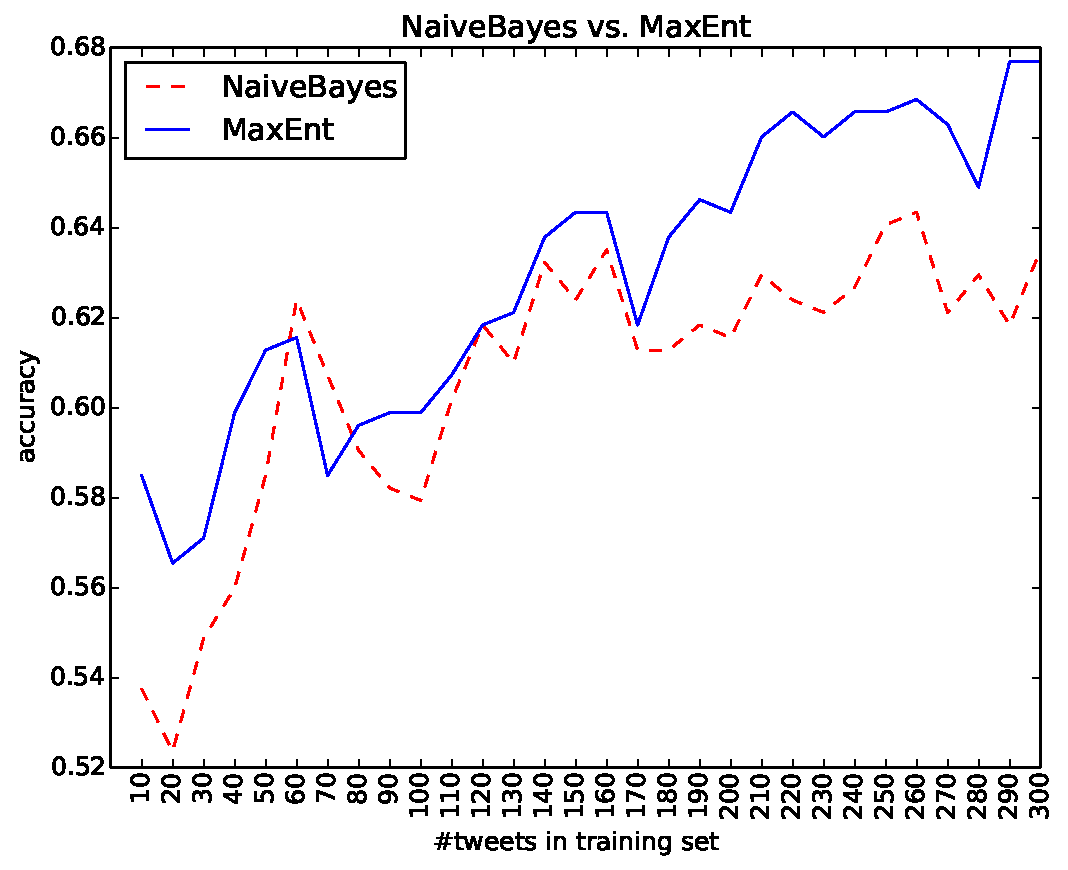
\includegraphics[width=0.9\textwidth]{bilder/cmp_nb_vs_me_S10_M300-16M.pdf}
\caption{Accuracy}
\label{img:acc}
\end{center}
\end{figure}

\begin{figure}[htbp]
\begin{center}
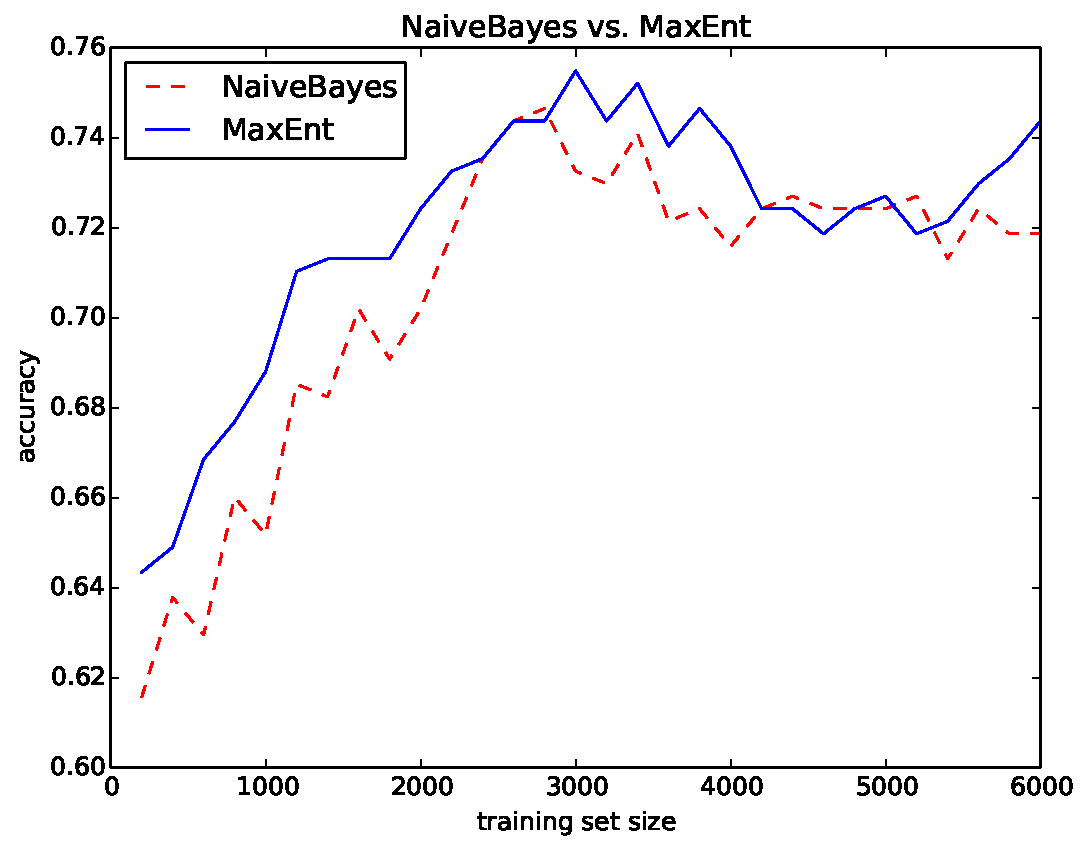
\includegraphics[width=0.75\textwidth]{bilder/cmp_nb_vs_me_S200_M6000.pdf}
\caption{Accuracy, Step 200}
\label{img:acc2}
\end{center}
\end{figure}

\begin{figure}[htbp]
\begin{center}
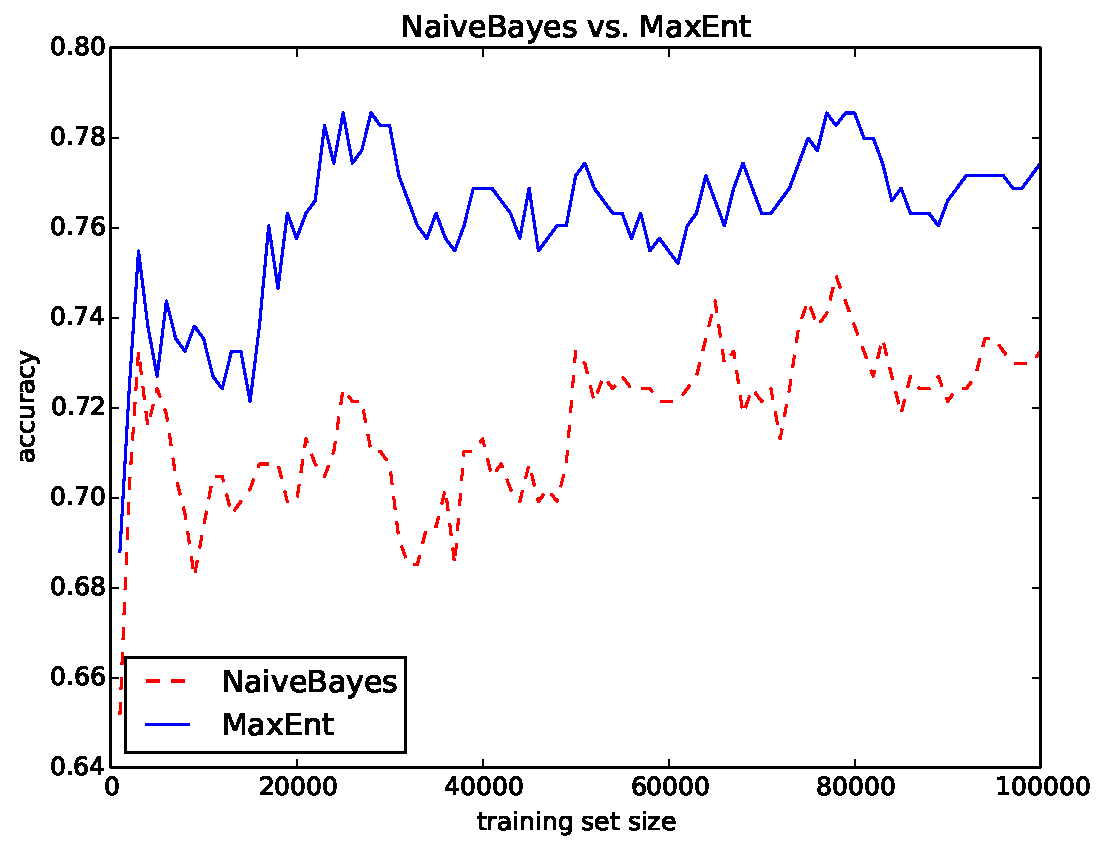
\includegraphics[width=0.75\textwidth]{bilder/cmp_nb_vs_me_S1000_M100000.pdf}
\caption{Accuracy, Step 1000}
\label{img:acc3}
\end{center}
\end{figure}


\section{Performancevergleich}
\section{Plot Stimmungsverlauf}


\chapter{Fazit}

\end{document}